\chapter{Absorber -- A New Approach to Monopole Interferometry}

If you were to wander onto almost any given radio telescope currently active in 
taking observations, you're almost certain to find some kind of reflective 
material underneath the antennas (either in the form of a ground screen or a 
reflective dish). One thing you're not likely to find is any kind of absorptive 
material -- we as astronomers are already fighting an uphill battle on 
attaining the very fine sensitivities needed to detect celestial sources, we 
really need all the photons we can get. 

However, in the case of a monopole interferometer, use of an absorber in your 
array design can actually be hugely beneficial, even despite the microscopic 
signal we aim to detect.

\section{Practical Instrumentation}

As discussed in Chapter~\ref{chap:interferometry}, one of the fundamental 
necessities of a monopole interferometer is close spacing of the antennas, in 
order to maximize reception of the global sky mode. However, this close spacing 
also predisposes the instrument to cross-talk. As discussed 
in~\citet{venumadhav2016}, this isn't necessarily a bad thing. Cross-talk is 
one of the ways that an array of antennas can maintain a sensitivity to the 
monopole -- each individual antenna will broadcast its reception of the 
monopole to its neighbors, and that reception will correlate. However, that 
also means that instrumental noise will be broadcast and correlated between 
antennas, vastly diminishing the useful properties of the interferometer and 
maintaining many of the pitfalls of single-dish instruments.

So we'd like to avoid cross-talk and other sources of correlated noise between 
elements as best as we can.

One way to manage that it to pack the space between antennas with absorber -- 
with a high-enough quality absorber, we can essentially make the antennas 
invisible to each other by just placing a tall enough wall between them.  
Ideally, this material would be quite thin, so that these absorber walls 
wouldn't force us to spread the shape of the array at all, thus maintaining a 
high sensitivity to the spatial monopole of the reionization global signal.

\section{Manipulating the Spatial Monopole}

Another huge benefit to the use of absorber in our array is how it can 
manipulate the instrument's sensitivity to the monopole. As discussed in 
Sec.~\ref{sec:observing-monopole}, by applying a spatial top-hat function to 
our monopole signal, we can increase our interferometric sensitivity to the 
global signal. The absorber can impose this top-hot function, by creating a 
spatial temperature change in the absorber's field of view.

\begin{figure}
    \begin{center}
    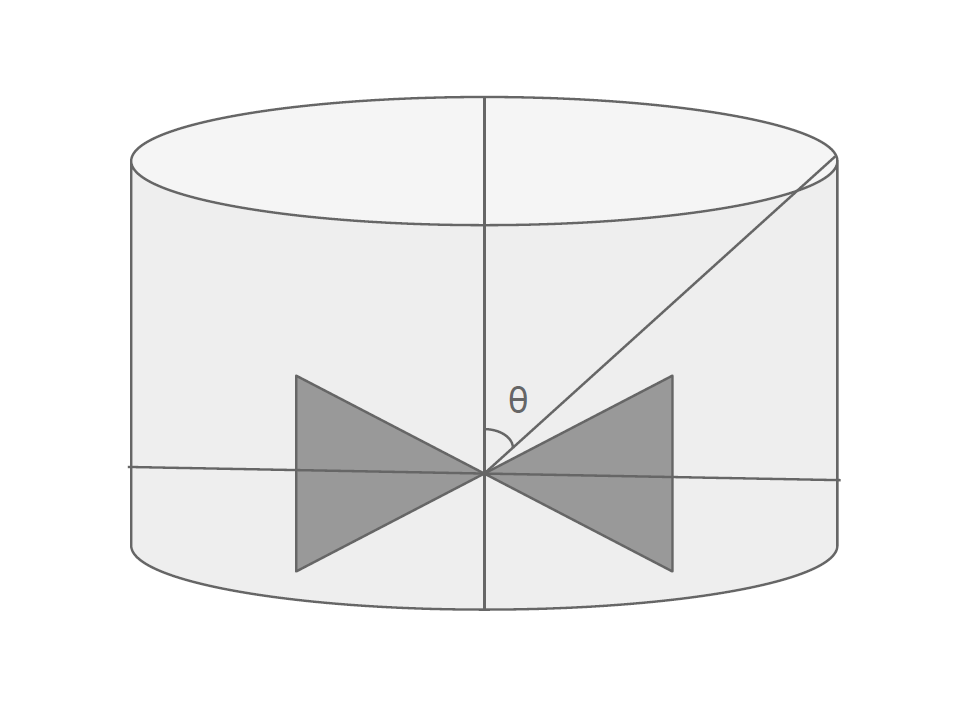
\includegraphics[width=\linewidth]{absorber-structure.png}
    \end{center}
    \caption{
        This cartoon shows the basic structure of the proposed absorber walls.  
        Each antenna in the array will be circled by a cylinder of absorber 
        material, creating a uniform temperature cutoff in the antenna's 
        reception of the sky. By increasing the height of the wall, we can 
        change the cutoff angle of the reception of the sky, thereby shrinking 
        the spatial top-hat and pushing more of the monopole to higher spatial 
        modes.
    }
    \label{fig:absorber-structure}
\end{figure}

Let's take a closer look at how this is to actually work. In a perfect world, 
our absorbing material would be $100\%$ effective and no information could be 
transmitted through it -- it would absorb all incident light and re-emit it as 
thermal radiation. That means that, as per Fig.~\ref{fig:absorber-structure} 
and ignoring the effects of the antenna beam shape, the antenna would see the 
sky up until an angle of $\theta$ off of zenith, and then it would see a 
perfect blackbody matching the ambient temperature of the array everywhere 
else.

One way to understand this would be to think in terms of optical depth, and the 
above case is one in which the absorber has an optical depth of $\tau = 
\infty$. This thinking also enables us to begin to understand more realistic 
scenarios, where we don't have perfect absorption between our antennas.

\begin{equation}
    I_{obs}(\theta) = I_{sky}~e^{-\tau_\theta} + S_{abs}~(1 - e^{-\tau_\theta})
    \label{eq:abs-optical-depth}
\end{equation}

In this quantitative construction of the reception of the array, we can see 
that the strength of the absorber determines the strength of the spatial cutoff 
-- particularly, in the case of a poor absorber, the above equation shows that 
there will be a great deal of sky leakage into the ``horizon". In particular, 
for reionization studies, this will be problematic due to the brightness of the 
sky at these frequencies from galactic synchrotron emission. So a weak absorber 
will barely put a dent in the sky brightness, diminishing the effectiveness of 
the imposed top-hat, and keeping the reionization global signal power in the 
lower, harder to detect spatial modes.

\section{Initial Results}

To date, we are still relatively early in the testing of our hypothesis that 
absorber walls or ``baffles" between antennas will enable us to better observe 
the spatial monopole with an interferometer. There have been two main sets of 
tests performed so far -- one in-lab test to measure the absorptivity of 
various proposed materials, and some brief field tests to gauge the 
effectiveness of our absorber at mitigating cross-talk between antennas.

The in-lab test was, in essence, a simple antenna return-loss measurement. To 
conduct the measurements, we started by constructing a large (i.e. 4.5' cube) 
Faraday cage out of wood and chicken wire, and placed an antenna at its center.  
From this setup, we could perform a simple return loss measurement and see what 
the maximum power return to the antenna is.

We could then line the cage with various absorptive materials and take another 
return-loss measurement, this time with (ideally) much of the power absorbed by 
the absorber, and see how effective each material is at dissipating energy 
within our science band. One such measurement is shown in 
Fig.~\ref{fig:fe-absorption}, featuring our most promising absorber candidate 
material, ferrite tiles.

\begin{figure}
    \begin{center}
    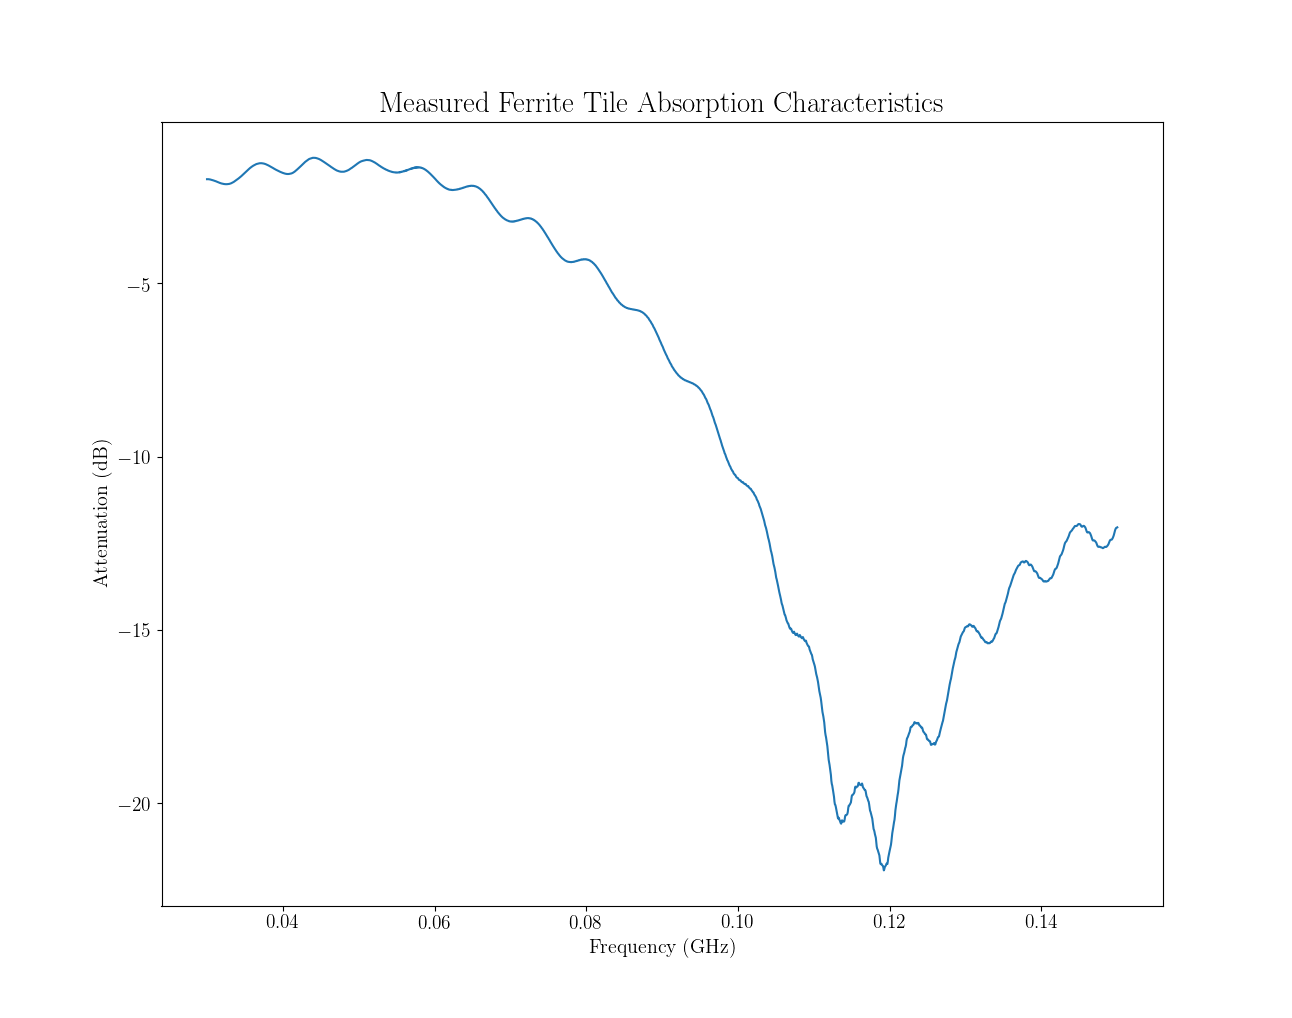
\includegraphics[width=\linewidth]{fe_absorption.png}
    \end{center}
    \caption{
        Here we see the results of a closed-box return loss measurement taken 
        with a densely packed (i.e. $9\times9$ tiles per wall) configuration of 
        ferrite tiles, evenly spaced along the walls of the testing Faraday 
        cage. The ripples are an artifact from the testing setup, and not 
        inherent to the performance of the ferrite itself. As can be easily 
        seen, the Ferrite performs much better at the high range of our science 
        band, and is optimized around $\sim120$ MHz.  While this material has 
        the best performance out of all the materials we have looked into so 
        far, we would ideally prefer a material with a more even absorptivity 
        across the band, so as best to avoid inadvertently adding ripples or 
        structure to our sky observations.
    }
    \label{fig:fe-absorption}
\end{figure}

As can be easily seen in the figure, the ferrite tiles have a decent 
absorptivity profile across the band, and an excellent absorptivity around 120 
MHz. However, as described in Section~\ref{sec:global-signal-overview}, the 
global signal of reionization is rich with physical information that is 
uniquely tied to its changing amplitude by frequency. The kinds of variations 
that we see in the absorptivity across the band are dangerous for the 
well-being of our experiment, as they could translate to tricky or uncertain 
calibration of our final instrument. We want to ensure that almost everything 
beyond the global signal has simple and well-defined relations to frequency 
(e.g. the synchrotron galactic sky, which is well described by a power law), in 
order to best understand our signal and be sure that instrumental 
idiosyncracies aren't being mistaken for true signal and science. As such, we 
would strongly prefer an absorber (or combination of absorbers) that has a more 
uniform performance across the science band.

Additionally, the ferrite tiles are among the most expensive of the materials 
we investigated. Even with a very close spacing and therefore relatively small 
baffle structures, the costs of acquiring enough ferrite to create an array 
quickly becomes overwhelming to the budget.
%\footnote{Of course, there's no longer any need to worry about that because 
%there is no budget -- this project dies alongside my academic ideals.}.

Other candidate absorbers include mats of Zotefoam Plastazote\textregistered, 
the AEP-EM low-frequency pyramidal foam absorber from DJM Electronics, and the 
creation of a grid of resistors designed to match with the free-space 
impedance~\citep{mahesh2015}. The Zotefoam was appealing due to its low cost 
compared to the pyramidal foam and ferrite tiles, but unfortunately its 
performance seemed to scale in proportion to its price tag.  The pyramidal foam 
performed slightly better, but seemed to feature more reflections than the 
ferrite and overall had a lower absorptivity performance than the ferrite, 
despite a nearly identical price tag per square foot of coverage. The resistive 
mesh is still an attractive idea, as it would only cost us an ungodly amount of 
effort to put together and about \$10 worth of resistors. Unfortunately, at the 
time of writing, only a very introductory level of investigation has been put 
into the resistive mesh idea, so nothing conclusive can be said about its 
performance as an absorber material.

At this point in time, there really haven't been any meaningful field tests 
upon which I could report. However, the most important things for us to 
investigate in the field would be a) ability of the absorber to mitigate the 
cross-talk between antennas and b) the efficacy of the baffles' ability to 
impose a spatial temperature variation from the antenna's point-of-view and how 
that efficacy evolves over frequency.

In Fig.~\ref{fig:field-test}, we see one possible arrangement of the absorber 
materials in order to assess the ability of the absorber at mitigating 
cross-talk between antennas. In order to perform this test adequately, one 
would need to take two measurements in the same radio environment -- one 
without the absorber between the antennas, in order to gauge the baseline level 
of cross-talk, and one with the absorber between, to measure the improvement in 
power leakage.

\begin{figure}
    \begin{center}
    \includegraphics[width=\linewidth]{field-test.png}
    \end{center}
    \caption{
        Shown here is a simple diagnostic field set-up that could be used to 
        evaluate an absorber's ability to mitigate cross-talk between elements.  
        Here we used a densely-packed configuration of ferrite tiles that have 
        been propped up on some of our pyramidal foam absorber for additional 
        height.
    }
    \label{fig:field-test}
\end{figure}
